В главе описан порядок разработки  педагогических инструментов, использующих интеллектуальных ассистентов. Глава разделена на секции 
\begin{itemize}
    \item анализ существующих инструментов повышения эффективности труда с использованием искуственного интеллекта
    \item разработка образовательных игр, обучающих использованию ассистентов 
\end{itemize}


Исследователи демонстрируют это через составления заданий количественно оценивающие способность моделей к выполнению арифметических операций, решения логических задач и созидательному творчеству. Текущий научный консенсус заключается в базовой неприменимости больших языковых моделей к этому спектру задач.

Тем не менее, уже сейчас модели показывают результаты, сопоставимые с человеком, на задачах перевода, пересказа и эмпатического понимания. Более того, современные техники работы с модель, включающие 
обучение на предметном корпусе 
интеграцию в управляющие системы
позволяют улучшить базовые показатели на десятки процентных пунктов.

\begin{figure}[h]
    \centering
    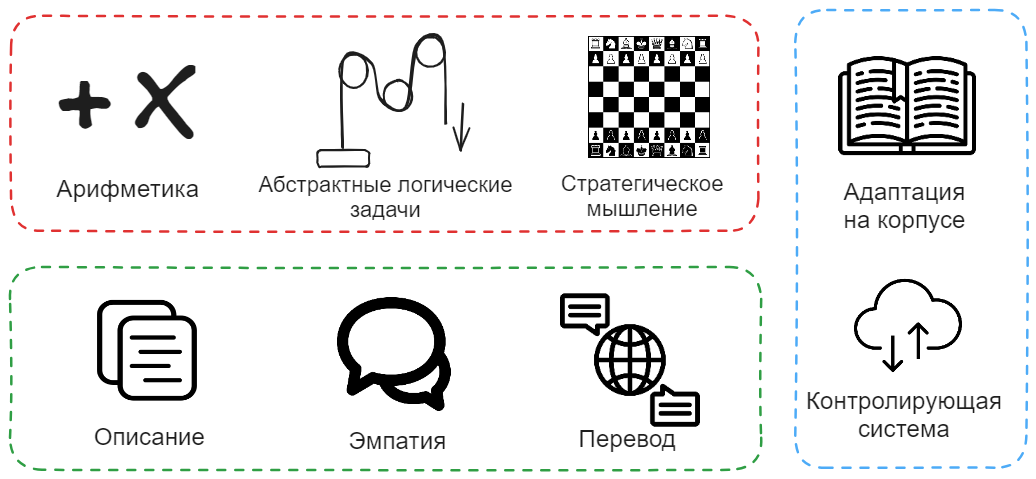
\includegraphics[width=0.5\textwidth]{assets/work/arch/problems.excalidraw.png}
    \caption{Этапы работы}
    \label{optimization}
\end{figure}
